%%%
%%%        Project: AraCom - Emotionale Robotik
%%%    Description: Introduction paper to emotional robotics
%%%        Version: 1.0
%%%         Author: Robert Jeutter <robert.jeutter@aracom.de>, Dennis Eisermann <dennis.eisermann@aracom.de>
%%%     Maintainer: Robert Jeutter <robert.jeutter@aracom.de>, Dennis Eisermann <dennis.eisermann@aracom.de>
%%%  Creation-Date: 24.05.2023
%%%      Copyright: (c) 2023 Robert Jeutter, Dennis Eisermann
%%%

\documentclass[aspectratio=169]{beamer}
%%%
%%%        Project: AraCom - LaTeX Template
%%%    Description: This is the basic LaTeX Template for all AraCom related presentations
%%%        Version: 1.0
%%%         Author: Robert Jeutter <robert.jeutter@aracom.de>
%%%     Maintainer: Robert Jeutter <robert.jeutter@aracom.de>
%%%  Creation-Date: 07.06.2023
%%%      Copyright: (c) 2023 Robert Jeutter
%%%      Images by AraCom IT Service
%%%

\usepackage{multirow}
\usepackage{subfigure}
\usepackage{etoolbox}
\usepackage{tikz}
\usepackage{listings}
\usepackage{graphicx}
\usepackage{xcolor}
\usepackage{amsfonts, amsmath, oldgerm, lmodern, animate}
\usepackage{verbatim}
\usepackage{bm}
\usefonttheme{serif}

\graphicspath{{./images/}}

\definecolor{aracomblue}{RGB}{38, 113, 142}
\definecolor{aracomred}{RGB}{143, 53, 70}
\definecolor{aracomgrey}{rgb}{0.9, 0.9, 0.9}

\setbeamercolor{block title}{fg=white,bg=aracomblue}
\setbeamercolor{block body}{fg=white,bg=aracomblue}

\newcommand{\themecolor}[1]{
		\setbeamercolor{normal text}{fg=darkgray,bg=white}
		\setbeamercolor{structure}{fg=aracomblue}
		\setbeamercolor{block title}{fg=aracomblue,bg=aracomgrey}
		\setbeamercolor{block body}{fg=darkgray,bg=aracomgrey}
}

\themecolor{white}
\setbeamercolor{title}{fg=aracomblue}
\setbeamercolor{alerted text}{fg=aracomred}
\setbeamercolor{author}{fg=black}
\setbeamercolor{date}{fg=black}

\setbeamerfont{author}{size=\scriptsize}
\setbeamerfont{date}{size=\tiny}
\setbeamerfont{title}{series=\bfseries}
\setbeamerfont{subtitle}{series=\mdseries,size=\footnotesize}
\setbeamerfont{frametitle}{series=\bfseries}
\setbeamerfont{framesubtitle}{series=\mdseries}
\setbeamerfont{block title}{series=\centering, size=\small}
\setbeamerfont{block body}{size=\scriptsize}

% Code to get prettier boxes
\setbeamertemplate{blocks}[rounded, shadow=true]

% Bullets in several levels
\setbeamertemplate{itemize item}{\textbullet}
\setbeamertemplate{itemize subitem}{\textemdash}
\setbeamertemplate{itemize subsubitem}{\ensuremath{\circ}}

\newenvironment{colorblock}[3][white]{%
	\begingroup
	\setbeamercolor{block title}{fg=#1,bg=#2}
	\setbeamercolor{block body} {fg=#1,bg=#2}
	\begin{block}{#3}
	}{%
	\end{block}
	\endgroup
}

% Put the logo in each slide's top left area
\pgfdeclareimage[width=0.1\paperwidth]{bluelogo}{./images/AraCom-Logo-black.png}
\renewcommand{\logo}{bluelogo}
\setbeamertemplate{headline}{\vspace{1ex}\hspace{0.03\textwidth}\pgfuseimage{\logo}}

% Define frame title and subtitle layout
\setbeamertemplate{frametitle}{
  \begin{beamercolorbox}[leftskip=2cm]{frametitle}%
    \usebeamerfont{frametitle}\insertframetitle\\
    \usebeamerfont{framesubtitle}\insertframesubtitle%
  \end{beamercolorbox}
}

% Define the title page
\setbeamertemplate{title page}{
  \vskip0pt plus 1filll
  \hspace{-12mm}% Pull back the box in an inelegant way - but it works!
  \begin{beamercolorbox}[wd=0.9\textwidth,sep=10pt,leftskip=8mm]{title}
    {\usebeamerfont{title}\inserttitle}

    {\usebeamerfont{subtitle}\insertsubtitle}

    {\usebeamerfont{author}\usebeamercolor[fg]{author}\insertauthor}

    {\usebeamerfont{date}\usebeamercolor[fg]{date}\insertdate}
  \end{beamercolorbox}
}

\newcommand{\TikzSplitSlide}[1]{%
  \rule{0.4\paperwidth}{0pt}%
  \begin{tikzpicture}
    \clip (-0.1\paperwidth,-0.5\paperheight) --
          ( 0.5\paperwidth,-0.5\paperheight) --
          ( 0.5\paperwidth, 0.5\paperheight) --
          ( 0.1\paperwidth, 0.5\paperheight) -- cycle;
    \node at (0.2\paperwidth,0) {%
      \includegraphics[height=\paperheight]{#1}%
    };
  \end{tikzpicture}
}

\renewcommand{\maketitle}{
\begingroup
  \setbeamertemplate{background}{
      \includegraphics[height=\paperheight]{./images/background.png}
  }
  \vspace{-5ex}\hspace{-5ex}\begin{frame}
      \Large\titlepage%
  \end{frame}
\endgroup
}

\newenvironment{chapter}[3][]{% Args: image (optional), color, frame title
  \begingroup
  \themecolor{blue}
  \ifstrequal{#2}{aracomlightgreen}{ % Use blue text on light green, else white
    \setbeamercolor{frametitle}{fg=aracomblue}
    \setbeamercolor{normal text}{fg=aracomblue,bg=#2}
  }{
    \setbeamercolor{frametitle}{fg=white}
    \setbeamercolor{normal text}{fg=white,bg=#2}
  }
  \ifstrempty{#1}{}{\setbeamertemplate{background}{\TikzSplitSlide{#1}}}
  \setbeamertemplate{frametitle}{%
    \vspace*{8ex}
    \begin{beamercolorbox}[wd=0.45\textwidth]{frametitle}
      \usebeamerfont{frametitle}\insertframetitle\\
      \usebeamerfont{framesubtitle}\insertframesubtitle%
    \end{beamercolorbox}
  }
  \begin{frame}{#3}
  \hspace*{0.05\textwidth}%
  \minipage{0.35\textwidth}%
  \usebeamercolor[fg]{normal text}%
}{%
  \endminipage%
  \end{frame}
  \endgroup
}

\newenvironment{sidepic}[2]{% Args: image, frame title
  \begingroup
  \setbeamertemplate{background}{%
  \hspace*{0.6\paperwidth}%
  \includegraphics[height=\paperheight]{#1}%
  }
  \setbeamertemplate{frametitle}{% Same as normal, but with right skip
    \vspace*{-3.5ex}
    \begin{beamercolorbox}[leftskip=2cm,rightskip=0.4\textwidth]{frametitle}%
      \usebeamerfont{frametitle}\insertframetitle\\
      \usebeamerfont{framesubtitle}\insertframesubtitle%
    \end{beamercolorbox}
  }
  \begin{frame}{#2}
  \minipage{0.6\textwidth}%
}{%
  \endminipage%
  \end{frame}
  \endgroup
}

\newcommand{\strtoc}{Table of Contents}
\newcommand{\strsubsec}{Section \thesection.\thesubsection}

% TYPESETTING ELEMENTS

% style of section presented in the table of contents
\setbeamertemplate{section in toc}{$\blacktriangleright$~\inserttocsection}

% style of subsection presented in the table of contents
\setbeamertemplate{subsection in toc}{}
% \setbeamertemplate{subsection in toc}{\footnotesize\hspace{1.2 em}$\blacktriangleright$~\inserttocsubsection}

% automate subtitle of each frame
\makeatletter
    \pretocmd\beamer@checkframetitle{\framesubtitle{\thesection\, \secname}}
\makeatother

% avoid numbering of frames that are breaked into multiply slides
\setbeamertemplate{frametitle continuation}{}

% at the begining of section, add table of contents with the current section highlighted
\AtBeginSection[]
{
    \begingroup
    \themecolor{blue}
    \begin{frame}{Table of Contents}
        \tableofcontents[currentsection]
    \end{frame}
    \endgroup
}

% at the beginning of subsection, add subsection title page
\AtBeginSubsection[]
{
    \begin{frame}{\,}{\thesection\, \secname}
        \fontfamily{ptm}\selectfont
        \centering\textsl{\textbf{\textcolor{aracomblue}{
            \large Section \thesection.\thesubsection%
            \vskip15pt
            \LARGE \subsecname%
        }}}
    \end{frame}
}

% code bolck setting
\definecolor{codegreen}{RGB}{101,218,120}
\definecolor{codegray}{rgb}{0.5,0.5,0.5}
\definecolor{codepurple}{rgb}{0.58,0,0.82}
\definecolor{backcolour}{rgb}{0.95,0.95,0.92}

\lstdefinestyle{mystyle}{
    % backgroundcolor=\color{backcolour},
    commentstyle=\color{aracomblue},
    keywordstyle=\color{magenta},
    numberstyle=\tiny\color{codegray},
    stringstyle=\color{codepurple},
    basicstyle=\ttfamily\scriptsize,
    breakatwhitespace=false,
    breaklines=true,
    captionpos=b,
    keepspaces=true,
    numbers=left,
    numbersep=5pt,
    showspaces=false,
    showstringspaces=false,
    showtabs=false,
    tabsize=4,
    xleftmargin=10pt,
    xrightmargin=10pt,
}

\lstset{style=mystyle}

% NEW COMMANDS

% set colored hyperlinks command
\newcommand{\hrefcol}[2]{\textcolor{aracomblue}{\href{#1}{#2}}}
\newcommand{\hlinkcol}[1]{\hrefcol{#1}{#1}}


% centering paragraph statement
\newcommand{\centerstate}[1]{
    \centering
    \begin{columns}
        \begin{column}{0.8\textwidth}
            #1
        \end{column}
    \end{columns}
}

% colored textbf
\newcommand{\atextbf}[1]{\textbf{\textcolor{aracomblue}{#1}}}
\newcommand{\atextsl}[1]{\textsl{\textcolor{aracomblue}{#1}}}
\newcommand{\aemph}[1]{\emph{\textcolor{aracomblue}{#1}}}

% about page
\newcommand{\aboutpage}[2]{
    \begingroup
    \themecolor{blue}
    \begin{frame}[c]{#1}{\,}
        \centering
        \begin{minipage}{\textwidth}
            \usebeamercolor[fg]{normal text}
            \centering
            \Large \textsl{\normalsize #2}
        \end{minipage}
    \end{frame}
    \endgroup
}

% bibliography page
\newcommand{\bibliographpage}{
    \section{References}

    \begingroup
    \themecolor{blue}
    \begin{frame}[allowframebreaks]{References}{\,}
        \tiny
        \printbibliography[heading=none]
    \end{frame}
\endgroup
}

\title{Emotionale Robotik}
\subtitle{Eine Einführung in die soziale Robotik}
\author{Robert Jeutter \& Dennis Eisermann}
\date{05. Oktober 2023}

\begin{document}

\maketitle

\section{Über uns}
\begin{frame}{Über uns}
  \begin{columns}
    \begin{column}{0.4\textwidth}
      \includegraphics[height=5cm]{images/robert.png}\\
      \textbf{Robert Jeutter}, 25, \arabar{}
      Softwareentwickler,\\
      \scriptsize{Schwerpunkte maschinelles Lernen und Mensch-Maschine-Interaktion}
    \end{column}
    \begin{column}{0.4\textwidth}
      \includegraphics[height=5cm]{images/dennis.png}\\
      \textbf{Dennis Eisermann}, 24, \arabar{}
      Softwareentwickler \& Masterand,\\
      \scriptsize{Schwerpunkte maschinelles Lernen und IT Security}
    \end{column}
  \end{columns}
\end{frame}
\begin{frame}{AraCom}
  \includegraphics[width=.6\linewidth]{images/AraCom-Logo-black.png}
  IT Service GmbH\\
  der Spezialist für maßgeschneiderte Software\\
  Hauptsitz in Gersthofen, weitere in München, Stuttgart und Bamberg\\
  bietet Spaß, Ausbildungsplätze \& spannende Projekte
\end{frame}
\begin{frame}{Sponsor des RoboCup}
  \includegraphics[height=30px]{images/AraCom-Logo-black.png} sponsort
  \includegraphics[height=35px]{images/RCJ_Logo.png}
  \begin{columns}
    \begin{column}{0.45\textwidth}
      \begin{figure}[h]
        \centering
        \includegraphics[width=\linewidth]{images/RoboCupFinale2023.jpg}
        %~ \cite{robocup} RoboCup Soccer Roboter
      \end{figure}
    \end{column}
    \begin{column}{0.45\textwidth}
      \begin{itemize}
        \item Robotik Wettbewerb
        \item Soccer, Rescue \& OnStage
        \item jährliche Austragung weltweit
        \item bis 2050 gegen Fifa Weltmeister
      \end{itemize}
    \end{column}
  \end{columns}
\end{frame}

\section{Emotionen}
\begin{frame}{Definition von Emotionen}
  \begin{itemize}
    \item Emotionen sind komplexe psychologische Zustände.
    \item Sie beinhalten drei unterschiedliche Komponenten:
          \begin{itemize}
            \item Ein subjektives Erleben.
            \item Eine physiologische Reaktion.
            \item Eine verhaltensbezogene oder expressive Antwort.
          \end{itemize}
    \item Emotionen sind vielschichtige Antworten auf Reize.
    \item Sie können durch unsere Umgebung oder Erinnerungen ausgelöst werden.
    \item Typischerweise von kurzer Dauer.
    \item Kann aus verbalen, physiologischen, verhaltensbezogenen und neuronalen Mechanismen bestehen.
  \end{itemize}
\end{frame}

\begin{frame}{Verhaltensbezogene oder expressive Emotionen}
  \begin{columns}
    \begin{column}{0.7\textwidth}
      \begin{itemize}
        \item Bezieht sich auf den sichtbaren Ausdruck von Emotionen.
        \item Gibt Hinweise über den emotionalen Zustand.
        \item Kommuniziert Absichten und Gefühle an andere.
        \item Beeinflusst soziale Interaktionen und Beziehungen.
        \item Kann automatisch oder bewusst gesteuert werden.
      \end{itemize}
    \end{column}
    \begin{column}{0.3\textwidth}
      \begin{figure}[h]
        \centering
        \includegraphics[width=\textwidth]{2020_EmotionWheel.png}
        \caption{Emotion Wheel}
      \end{figure}
    \end{column}
  \end{columns}
\end{frame}

\begin{frame}{Emotionen auszudrücken}
  \begin{columns}
    \begin{column}{0.7\textwidth}
      \begin{itemize}
        \item<1-> Gesichtsausdrücke, z.B. Lächeln oder Stirnrunzeln.
        \item<2-> Gesten, z.B. Klatschen oder Zeigen.
        \item<3-> Körpersprache, z.B. Körperhaltung oder Nähe.
        \item<4-> Stimmklang, z.B. Schreien oder Flüstern.
      \end{itemize}
    \end{column}
    \begin{column}{0.3\textwidth}<1>
      \begin{figure}[h]
        \centering
        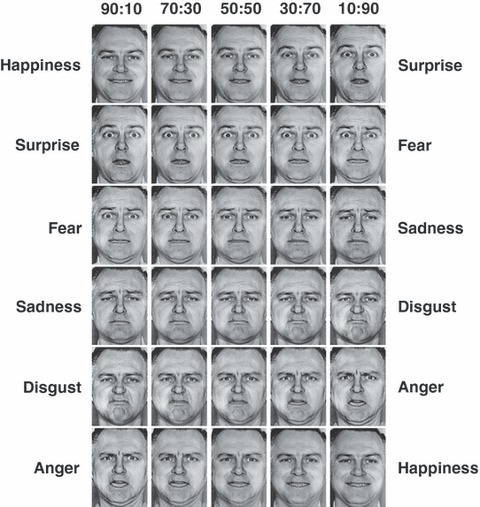
\includegraphics[width=\textwidth]{Facial-expression-continua-used-in-the-Emotion-Hexagon-task-Running-from-left-to-right.jpeg}
        \caption{facial Expressions~\cite{facialExpressionRecognition} }
      \end{figure}
    \end{column}
    \begin{column}{0.3\textwidth}<3->
      \begin{figure}[h]
        \centering
        \includegraphics[width=\textwidth]{Canine-Body-Language.png}
        \caption{Dog Language~\cite{doggieLanguage} }
      \end{figure}
    \end{column}
  \end{columns}
\end{frame}

\begin{frame}{Definition --- Soziale und Emotionale Intelligenz}
  \textbf{Definition sozialer Intelligenz}
  \begin{quote}
    Verstehen und Navigieren in sozialen Umgebungen und Interaktionen.
  \end{quote}
  \vspace{1cm}

  \textbf{Definition emotionaler Intelligenz}
  \begin{quote}
    Erkennen, Verstehen und Steuern der eigenen Emotionen\\
    sowie der Emotionen anderer.
  \end{quote}
\end{frame}

\section{Emotionen in der Robotik}
\begin{frame}{Verschmelzende Domänen bei emotionaler Robotik}
  \begin{center}
    Robotik\\
    +\\
    Psychologie\\
    +\\
    Künstlicher Intelligenz
  \end{center}
\end{frame}

\begin{frame}{Aufstieg der Emotionalen Robotik}
  \textbf{Ursprünge der emotionalen Robotik}
  \begin{itemize}
    \item Erkennen menschlicher Emotionen
    \item Reagieren und Interagieren auf Basis dieser Emotionen
  \end{itemize}

  \textbf{Aktueller Stand}
  \begin{itemize}
    \item Emotionserkennung
    \item Feedback-Mechanismen
    \item Anwendungen in realen Szenarien
  \end{itemize}
\end{frame}

\begin{frame}{Ziele und Vorteile der Emotionalen Robotik}
  \begin{columns}
    \begin{column}{0.7\textwidth}
      \textbf{Hauptziele}
      \begin{itemize}
        \item Vertiefung der Mensch-Maschine-Interaktionen
        \item Personalisierte Benutzererfahrungen
      \end{itemize}

      \textbf{Wesentliche Vorteile}
      \begin{itemize}
        \item Emotionaler Support
        \item Motivation und Ansporn
        \item Steigerung der Geselligkeit
        \item Verbesserung der Lebensqualität
      \end{itemize}
    \end{column}
    \begin{column}{0.3\textwidth}
      \begin{figure}[h]
        \centering
        \includegraphics[width=\textwidth]{andy-kelly-0E_vhMVqL9g-unsplash.png}
        \caption{Mensch \& Roboter Interagieren}
      \end{figure}
    \end{column}
  \end{columns}
\end{frame}

\begin{frame}{Risiken und Bedenken}
  \begin{itemize}
    \item Datenschutz und -sicherheit
    \item Emotionale Manipulation durch Maschinen
    \item Potenzielle Voreingenommenheiten bei der Emotionserkennung
  \end{itemize}
\end{frame}

\section{Einsatz emotionaler Robotik}
\begin{frame}{Anwendungen und Einsatzmöglichkeiten}
  \textbf{Aktuelle Einsatzbereiche}
  \begin{itemize}
    \item Therapeutische Umgebungen
    \item Kundenservice
  \end{itemize}
  \vspace{1cm}

  \textbf{Potenzielle Bereiche}
  \begin{itemize}
    \item Pflege von älteren Menschen
    \item Unterstützung der psychischen Gesundheit
    \item Personalisiertes Tutoring
  \end{itemize}
\end{frame}

\begin{frame}{Einführung von Emotionaler Robotik im Betrieb}
  \textbf{Technologische Anforderungen}
  \begin{itemize}
    \item Robotik: Sensoren, Prozessoren, Aktoren
    \item ML-Modelle: Umgebungserkennung, Schlussfolgern
  \end{itemize}
  \vspace{.5cm}

  \textbf{Training und Datenerfassung}
  \begin{itemize}
    \item Erfassung emotionaler Daten
    \item Verfeinerung von Maschinenantworten
    \item Feedback-Schleifen zwischen Mensch und Maschine
  \end{itemize}
  \vspace{.5cm}

  \textbf{Ethische Anforderungen}
  \begin{itemize}
    \item Richtlinien und Vorsichtsmaßnahmen für Unternehmen
    \item Akzeptanz von maschinellen Lösungen schaffen
    \item Differenz zwischen Mensch und Maschine
  \end{itemize}
\end{frame}

\begin{frame}{Zukünftige Horizonte}
  \begin{itemize}
    \item Fortgeschrittene Modelle, die kulturelle Unterschiede berücksichtigen
    \item Roboter, die künstliche Empathie zeigen
    \item Generierung und Ausdruck einzigartiger Roboter-,,Emotionen''
  \end{itemize}
\end{frame}

\begin{frame}{Anthropomorphismus und Vertrauen}
  \begin{columns}
    \begin{column}{.5\textwidth}
      \textbf{Anthropomorphismus}: Zuweisung menschlicher Eigenschaften
    \end{column}
    \begin{column}{.5\textwidth}
      \begin{figure}[h]
        \centering
        \includegraphics[width=.6\textwidth]{2h-media-L3BtJiiSkwY-unsplash.png}
        \caption{Mensch \& Roboter Interagieren}
      \end{figure}
    \end{column}
  \end{columns}

  \textbf{Die Implikationen für Roboter}
  \begin{itemize}
    \item Erhöhtes Vertrauen
    \item ,,Uncanny Valley'' Effekt
  \end{itemize}
  \vspace{.5cm}

  \textbf{Herausforderungen}
  \begin{itemize}
    \item Ängste im Zusammenhang mit Technologie ansprechen
    \item Akzeptanz fördern
  \end{itemize}

\end{frame}

\begin{frame}{,,Uncanny Valley'' Effekt}
  \begin{itemize}
    \item Konzept in Robotik und Animation.
    \item Unbehagen durch fast-menschliche Darstellung.
    \item 1970 von Masahiro Mori geprägt.
    \item Höchstes Unwohlsein vor perfekter Menschlichkeit.
    \item Beeinflusst Technologieakzeptanz.
  \end{itemize}
\end{frame}

\section{Zusammen-fassung}
\begin{frame}{Schlussfolgerung und Schlüsselerkenntnisse}
  \begin{itemize}
    \item Zusammenfassung des Potenzials und der Herausforderungen der emotionalen Robotik
    \item Ermutigung zur weiteren Erkundung und zum Verständnis in diesem Bereich
    \item Einladung zu Zusammenarbeiten und Diskussionen nach der Präsentation
  \end{itemize}
\end{frame}

\begin{frame}{Danksagungen}
  \begin{itemize}
    \item \textbf{Aracom IT Services GmbH} für die Unterstützung bei der Erstellung dieser Präsentation
    \item \textbf{Hackerkiste} für die Organisation dieses tollen Events
  \end{itemize}
\end{frame}

\begin{frame}[c]{}
  \centering
  \begin{minipage}{\textwidth}
    \usebeamercolor[fg]{normal text}
    \centering
    \Large \atextsl{Alle Folien als CC-BY-SA verfügbar auf}\\
    \href{https://github.com/wieerwill/emotional-robotics}{GitHub.com/WieErWill/emotional-robotics}\\
    \vspace{.4cm}
    \includegraphics[width=.4\linewidth]{images/qrcode-repo.png}
  \end{minipage}
\end{frame}

\begin{frame}[c]{}
  \centering
  \begin{minipage}{\textwidth}
    \usebeamercolor[fg]{normal text}
    \centering
    \Huge \[\mathcal Q \& \mathcal A\]
    \Large \atextsl{
      Vielen Dank für eure Aufmerksamkeit! \\
      Feedback und Diskussionen sind sehr willkommen \\
    }
  \end{minipage}
\end{frame}

\section{Quellen \& Literatur}
\begin{frame}[allowframebreaks]{Quellen \& Literatur}
  \scriptsize
  \bibliography{../bibliography}
  \bibliographystyle{unsrt}
\end{frame}

\end{document}